
\documentclass[conference]{IEEEtran}
\IEEEoverridecommandlockouts
\renewcommand{\thesection}{\Roman{section}}
\usepackage{booktabs}
\usepackage{fancyhdr}
\usepackage[usenames, dvipsnames]{xcolor}
\usepackage{colortbl}
\usepackage{caption}
\usepackage{graphicx}
\usepackage{array}
\usepackage{adjustbox}
\usepackage{hyperref,graphicx,color,float}
\definecolor{myblue}{RGB}{10, 150, 200}

\usepackage{cite}
\usepackage{multirow}
\usepackage{amsmath,amssymb,amsfonts}
\usepackage{algorithmic}
\usepackage{graphicx}
\usepackage{textcomp}
\usepackage{comment}
\definecolor{highlightColor}{HTML}{E6FFE6}

% --- packages required by this paper's figures and algorithm ---
\usepackage[ruled,vlined]{algorithm2e}
\usepackage{enumitem}
\usepackage{subcaption}
\usepackage{tikz}
\usetikzlibrary{positioning,arrows.meta,shapes.geometric,calc,fit,backgrounds}
\usepackage{pgfplots}
\pgfplotsset{compat=1.17}
\usepgfplotslibrary{groupplots}
\definecolor{beforeblue}{RGB}{31,119,180}
\definecolor{afterorange}{RGB}{255,127,14}

\usepackage{xcolor}
\def\BibTeX{{\rm B\kern-.05em{\sc i\kern-.025em b}\kern-.08em
    T\kern-.1667em\lower.7ex\hbox{E}\kern-.125emX}}

\pagestyle{empty}

\title{Tackling Entangled Enhancement in the Model\\
Pipeline for Autonomous Vehicles}

\author{\IEEEauthorblockN{Rashedul Arefin Ifty, Fumio Machida}
\IEEEauthorblockA{University of Tsukuba\\
Tsukuba, Japan\\
ifty.rashedul@sd.cs.tsukuba.ac.jp, machida@cs.tsukuba.ac.jp}}

\begin{document}
\maketitle
\thispagestyle{empty}
\bstctlcite{IEEEexample:BSTcontrol}% disable em-dash for repeated author names

\begin{abstract}
Autonomous Vehicles (AVs) are increasingly built as a pipeline of separately trained
perception, prediction, and planning models. Each model in the pipeline is often maintained separately when it needs to be updated. However, retraining a single upstream model
can cause performance degradation in the downstream models due to distribution shift. Although such a failure is known as entangled enhancement, the phenomenon in the AV pipeline has not been widely investigated. In this paper, we first formally define entangled enhancement in the perception--prediction--planning pipeline by separating a model's own error from the error inherited from upstream models. We then empirically demonstrate real entangled enhancement in an AV pipeline built from the nuScenes dataset, by analyzing the impact of the retrained perception model across a geographic domain shift on the downstream prediction and planning models. Across $15$
retraining updates that vary the dataset size, the training epochs, and the random seed, the perception model improves its perception accuracy every time. However, $6$ of them increase the L2 displacement error of the planning model output, exhibiting real entangled enhancement. To proactively mitigate entangled enhancement in the AV pipeline, we propose Cascade-Aware Retraining Assessment
(CARA), which guides the decision to adopt the retrained model by measuring the performance difference between the isolated mode and the upstream-dependent mode. Our evaluation with the nuScenes retraining scenario shows that CARA can effectively identify the symptoms of entangled enhancement and can provide a meaningful precaution before adopting the updated model in the pipeline.
\end{abstract}

\begin{IEEEkeywords}
autonomous driving, cascade effects, machine learning systems, model pipelines,
regression testing, retraining, software reliability
\end{IEEEkeywords}

% ============================================================================
\section{Introduction}
% ============================================================================
Autonomous Vehicles (AVs) are increasingly built as a pipeline of separately trained
perception, prediction, and planning models. Perception detects the surrounding agents,
prediction forecasts their motion, and planning selects the driving
trajectory~\cite{chen2024e2esurvey,hu2023uniad}. In deployment, such a pipeline
is maintained under domain drift one model at a time. A perception model is
retrained for a new city, a prediction model is updated when traffic changes, and a planning model is revised for new regulations. This kind of maintenance is possible only in a pipeline. Each model can be retrained on its own. In an end-to-end network the whole network must be retrained at once. We therefore adopt the pipeline as the setting for this study.

\looseness=-1
In practice, one model is usually retrained while the others stay fixed. This is where a problem can appear. The retrained model becomes better on its own metric, but the models after it become worse. The reason is that those models were built and evaluated on the output of the earlier version of the retrained model. The first reported
instance of this self-defeating behavior appeared in an object-detection setting
\cite{wu2021fixesthatfail}, where a better detector reduced the
accuracy of the downstream task. Wang and Machida~\cite{wang2024compsac} modeled and analyzed entangled enhancement in a two-model machine learning system by a
continuous-time Markov chain. Entangled enhancement has also been reported in a
sentence-classification system~\cite{wang2025issre}. Sculley et al.~\cite{sculley2015hidden} describe the same difficulty more generally. When learning components depend on each other, changing one of them creates maintenance problems for the others. However, no existing study examines entangled
enhancement across an entire perception--prediction--planning pipeline for
AVs. Although previous studies also consider the perception module of an AV, their analysis was limited to two sequential models and focused only on the perception component.

\looseness=-1
To address this gap, this paper studies how a single-model retraining event
propagates through an AV pipeline, using empirical analysis. For the empirical analysis, we build a three-model pipeline on the nuScenes
dataset~\cite{caesar2020nuscenes}. The perception model is
YOLOv11n~\cite{jocher2024yolo11}, an object detector applied to the front-camera
image. The prediction model is a constant-velocity trajectory predictor. The
planning model is a rule-based planner from the Intelligent Driver Model (IDM)
family~\cite{treiber2000idm}, whose proposal-and-score design follows
PDM-Closed~\cite{dauner2023parting}. We train the perception model on Boston
scenes and fine-tune it on Singapore scenes, a well-known domain gap within
nuScenes, and investigate how the updates impact the downstream performance. To separate a
model's own error from the error it inherits from upstream, each downstream model
is measured in two modes, one with ground-truth inputs and one with the live
upstream output. Because a single retraining is only one data point, we run a
campaign of $15$ retraining updates that vary the amount of fine-tuning data, the
number of training epochs, and the random seed.

\vspace{2pt}
This paper makes three contributions.
\begin{itemize}[leftmargin=*, itemsep=2pt, topsep=2pt]
\item We formally define entangled enhancement in the
perception--prediction--planning pipeline for AVs, and introduce the cascade coupling factor that quantifies the intensity of entangled enhancement.

\item We empirically investigate real entangled enhancement in an AV pipeline generated from the nuScenes dataset, showing that six out of $15$ retraining trials exhibit entangled enhancement.
\item We propose a retraining assessment framework, CARA, which can evaluate potential entangled enhancement by measuring the performance difference between the isolated mode and the upstream-dependent mode.
\end{itemize}

The remainder of the paper is organized as follows.
Section~\ref{sec:method} formalizes the pipeline model and the definition of
entangled enhancement. Section~\ref{sec:cara} presents the proposed CARA method.
Section~\ref{sec:setup} details the experimental setup and the retraining
campaign. Section~\ref{sec:results} reports the empirical evidence of entangled
enhancement and the evaluation of CARA.
Section~\ref{sec:implications} discusses the mechanism and its implications,
Section~\ref{sec:related} reviews related work, and
Section~\ref{sec:conclusion} concludes.

% ============================================================================
\section{System Model and Methodology}
\label{sec:method}
% ============================================================================

\subsection{Formal Pipeline Model}
We model an AV pipeline as a composition of three functions,
\begin{equation}
S = C_1 \circ C_2 \circ C_3,
\qquad
S(x) = C_3\bigl(C_2(C_1(x))\bigr),
\label{eq:comp}
\end{equation}
where $x$ is an input camera frame processed through the three models:
\begin{itemize}
\item \textbf{Perception ($C_1$).} The output $z_1 = C_1(x)$ is a list of the objects the model found in the image. For each object it gives the type, the size, and the position on the road around our own car.
\item \textbf{Prediction ($C_2$).} The output $z_2 = C_2(z_1)$ is, for every
detected object, a forecast trajectory over the next several seconds.
\item \textbf{Planning ($C_3$).} The output $z_3 = C_3(z_2)$ is the ego vehicle's
planned trajectory, a sequence of positions over a $3$~s horizon.
\end{itemize}
The outputs $z_1$ and $z_2$ connect one model to the next. A change in $C_1$
therefore changes $z_1$, which is the input of $C_2$. The change then reaches
$z_2$, which is the input of $C_3$. Now suppose that only $C_1$ is retrained. The
parameters of $C_2$ and $C_3$ are unchanged. Any change in their outputs
therefore comes only from their inputs.

\subsection{Entangled Enhancement}
\label{sec:ee-def}
Entangled enhancement occurs when an upstream model is retrained and improves its own performance, and yet the system as a whole degrades~\cite{wang2024compsac}.
This entanglement happens because the downstream models were tuned to the
statistics of the \emph{original} upstream output and are shifted after the upstream model update. We denote by $\delta_1$ the improvement of the perception performance of
$C_1$ after retraining, and by $\Delta_3$ the
degradation of the planning performance of $C_3$. Entangled enhancement is formally specified by the joint condition
\begin{equation}
\underbrace{\delta_1 > 0}_{C_1\ \text{improves}}
\ \wedge\
\underbrace{\Delta_3 > 0}_{\text{system degrades}} .
\label{eq:ee}
\end{equation}
The condition requires the upstream model to improve on its \emph{own} performance
($\delta_1 > 0$) while the system nonetheless degrades ($\Delta_3 > 0$). The upstream model must improve for this to be entangled enhancement. If the upstream model became worse and the system became worse with it, that is an ordinary regression.

\subsection{Cascade Gap and the Isolation Property}
\label{sec:dualmode}
To make entangled enhancement measurable, we separate a model's own error from
the error inherited from the upstream models. Let $z_k$ denote the output of model $C_k$,
and let $M_k(z_k)$ be an error metric evaluated on that output, with lower values
better. We evaluate each downstream model in two modes. In \emph{isolated} mode a
model receives ground-truth inputs, and its output is written $z_k^{\text{iso}}$.
For $C_2$ and $C_3$,
\begin{align}
z_2^{\text{iso}} &= C_2(z_1^{\star}), &
z_3^{\text{iso}} &= C_3(z_2^{\star}),
\label{eq:iso-mode}
\end{align}
where $z_k^{\star}$ is the ground-truth value of $C_k$. In \emph{pipeline}
mode a model receives the direct output of the upstream neighbor, and its output is
written $z_k^{\text{pipe}}$,
\begin{align}
z_2^{\text{pipe}} &= C_2(C_1(x)), &
z_3^{\text{pipe}} &= C_3(C_2(C_1(x))).
\label{eq:pipe-mode}
\end{align}
The metric in isolated mode, $M_k(z_k^{\text{iso}})$, reflects the model's own
error, while the metric in pipeline mode, $M_k(z_k^{\text{pipe}})$, reflects its
own error together with the error inherited from the upstream model. The difference between
the two is the inherited part, which we call the \emph{cascade gap} at $C_k$,
\begin{equation}
\Gamma_k = M_k(z_k^{\text{pipe}}) - M_k(z_k^{\text{iso}}).
\label{eq:gap}
\end{equation}
Isolated mode needs ground-truth inputs. It can therefore be run only in an experiment, not in a real vehicle. It shows whether a change came from the model itself or from its input.

Consider a retraining event that replaces an upstream model $C_k$ by an updated
model $C_k'$, whose outputs we write $z_k'$. If the pipeline is properly composed,
the retraining leaves the isolated-mode output of every downstream model that was
not retrained unchanged, because that output depends only on the ground-truth
inputs. We call
this the \emph{isolation property},
\begin{equation}
M_k(z_k^{\text{iso}}) = M_k(z_k^{\text{iso}\,\prime})
\label{eq:iso}
\end{equation}
Equation~\eqref{eq:iso} is a testable property of the setup rather than an
assumption. Any change in the isolated-mode metric of a model that was not retrained indicates
contamination, and we verify the equation in Section~\ref{sec:results}. The effect
that the retraining causes at model $C_k$ is the change in its pipeline
metric,
\begin{equation}
\Delta_k = M_k(z_k^{\text{pipe}\,\prime}) - M_k(z_k^{\text{pipe}}),
\label{eq:inj}
\end{equation}
which, given~\eqref{eq:iso}, equals the change in the cascade gap $\Gamma_k$.

\subsection{Coupling Factor}
\label{sec:diag}
To quantify the intensity of entangled enhancement, we relate the system performance degradation $\Delta_3$ to the upstream
improvement $\delta_1$, through the \emph{cascade coupling
factor}
\begin{equation}
\rho_{1\to 3} = \frac{\Delta_3}{\delta_1}.
\label{eq:rho-def}
\end{equation}
Under the sign convention above, a positive $\delta_1$ improves the upstream model
and a positive $\Delta_3$ worsens the system. Entangled enhancement therefore
corresponds to $\rho_{1\to 3} > 0$, and its magnitude measures how much regression
of the planning metric accompanies a unit of upstream improvement. The factor is well defined whenever
$\delta_1 \neq 0$. As Section~\ref{sec:results} shows, the retraining campaign
enters the entangled-enhancement regime in $6$ of $15$ updates, for which
$\rho_{1\to 3} > 0$ is read together with the full effect vector
$(\Delta_2, \Delta_3)$ rather than as an isolated scalar.

% ============================================================================
\section{Cascade-Aware Retraining Assessment}
\label{sec:cara}
% ============================================================================
The formal definition of Section~\ref{sec:method} exposes a concrete hazard for
maintenance. An updated model that improves on its own metric, and even improves
the metric of its immediate consumer, can still degrade the planning output.
Neither a check on the updated model alone nor a check on the next model alone is
therefore a sufficient criterion for admitting the update. We turn the definition
into an admission check for model updates, Cascade-Aware Retraining Assessment
(CARA). CARA is an explicit gate that measures the effect of an update at every
downstream model and admits the update only when the effect on the planning metric
stays within a threshold. Fig.~\ref{fig:cara} summarizes the decision and
Algorithm~\ref{alg:cara} states it.

\begin{figure}[htbp]
\centering
\resizebox{\columnwidth}{!}{%
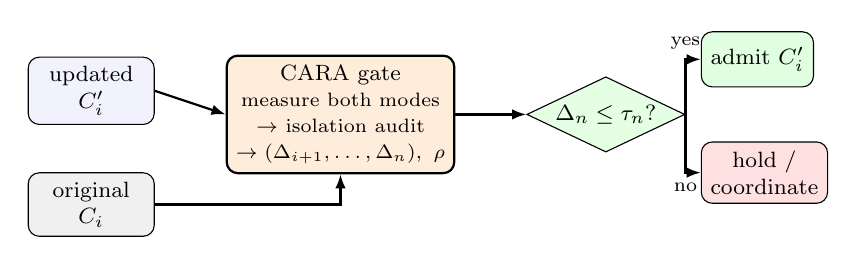
\begin{tikzpicture}[
    font=\footnotesize,
    node distance=5mm,
    box/.style={draw, rounded corners, minimum height=7mm, minimum width=16mm,
                align=center, fill=blue!5},
    old/.style={draw, rounded corners, minimum height=7mm, minimum width=16mm,
                align=center, fill=black!6},
    gate/.style={draw, rounded corners, minimum height=10mm, minimum width=26mm,
                 align=center, fill=orange!14, thick},
    dec/.style={draw, diamond, aspect=2.1, align=center, fill=green!10, inner sep=1pt},
    pass/.style={draw, rounded corners, minimum height=7mm, align=center, fill=green!12},
    stop/.style={draw, rounded corners, minimum height=7mm, align=center, fill=red!12},
    arr/.style={-{Latex[length=1.8mm]}, thick}
]
\node[box] (new) {updated\\$C_i'$};
\node[old, below=6mm of new] (old) {original\\$C_i$};
\node[gate, right=9mm of new, yshift=-3mm] (gate)
     {CARA gate\\\scriptsize measure both modes\\\scriptsize $\to$ isolation audit\\\scriptsize $\to (\Delta_{i+1},\dots,\Delta_n),\ \rho$};
\node[dec, right=9mm of gate] (dec) {$\Delta_n \le \tau_n$?};
\node[pass, above right=1mm and 7mm of dec] (pass) {admit $C_i'$};
\node[stop, below right=1mm and 7mm of dec] (stop) {hold /\\coordinate};
\draw[arr] (new.east) -- (gate.west);
\draw[arr] (old.east) -| ($(gate.south)$);
\draw[arr] (gate) -- (dec);
\draw[arr] (dec.east) |- (pass.west) node[midway,above,font=\scriptsize]{yes};
\draw[arr] (dec.east) |- (stop.west) node[midway,below,font=\scriptsize]{no};
\end{tikzpicture}%
}
\caption{The CARA admission check for an updated model.}
\label{fig:cara}
\end{figure}

\subsection{The Admission Procedure}
The inputs to CARA are a pipeline $C_1 \to \dots \to C_n$, an audit set $A$, a
candidate update that replaces the original model $C_i$ by an updated model
$C_i'$, and a threshold $\tau_n$ on the metric of the last model. The audit set is a fixed collection of
driving scenes, annotated with the ground truth that the isolated mode requires.
Holding $A$ fixed makes the two evaluations comparable, because $C_i$ or $C_i'$ is
then the only difference between them. CARA produces an admit-or-hold decision, the
change at every downstream model, and the coupling factor. The procedure has three
steps, shown in Fig.~\ref{fig:cara} and stated in Algorithm~\ref{alg:cara}.

The first step measures both models on the same audit set. CARA runs the two-mode
measurement of Section~\ref{sec:dualmode} on $A$ with $C_i$ in place, then repeats
it with $C_i'$ in place under the same seeds. Each run records, for every
downstream model, its metric in isolated mode and its metric in pipeline mode.

The second step checks the isolation property~\eqref{eq:iso}. For every
downstream model $C_k$ with $k>i$, which was not retrained, the isolated-mode
metric must be identical before and
after the update, because that metric depends only on ground-truth inputs. A
difference indicates leakage or nondeterminism and makes the assessment invalid.
This check is what allows any measured change to be attributed to the update.

The third step computes the change at each model and decides. For every downstream
model $C_k$, CARA computes the change in its pipeline-mode metric $\Delta_k$
from~\eqref{eq:inj}. CARA then reports all of these changes together, as
$(\Delta_{i+1}, \dots, \Delta_n)$. Two neighbouring models can move in opposite
directions, which a single summary number would hide. CARA also reports the coupling factor
$\rho_{i\to n} = \Delta_n / \delta_i$, whose sign identifies entangled enhancement
under the convention of Section~\ref{sec:ee-def}. The update is admitted only when the effect on the last
model stays within the threshold, $\Delta_n \le \tau_n$, and the collision rate does
not become worse. Otherwise the update is held, and the
downstream consumers are retrained together with it.

\begin{algorithm}[htbp]
\SetAlgoLined
\DontPrintSemicolon
\KwIn{pipeline $C_1\!\to\!\dots\!\to\!C_n$, audit set $A$, original model $C_i$,
updated model $C_i'$, threshold $\tau_n$}
\KwOut{admit or hold decision, the changes $(\Delta_{i+1},\dots,\Delta_n)$,
coupling factor $\rho$}
Measure both modes with $C_i$ on $A$, giving $M_k(z_k^{\text{iso}})$ and
$M_k(z_k^{\text{pipe}})$ for every downstream $C_k$\;
Measure both modes with $C_i'$ on $A$ under the same seeds, giving
$M_k(z_k^{\text{iso}\,\prime})$ and $M_k(z_k^{\text{pipe}\,\prime})$\;
\ForEach{downstream $C_k$ with $k>i$}{
  \If{$M_k(z_k^{\text{iso}}) \ne M_k(z_k^{\text{iso}\,\prime})$}{
    \Return \textbf{invalid} \tcp*{isolation violated}
  }
}
$\Delta_k \leftarrow M_k(z_k^{\text{pipe}\,\prime}) - M_k(z_k^{\text{pipe}})$
\quad for $k=i{+}1,\dots,n$\;
$\rho \leftarrow \Delta_n / \delta_i$\;
\eIf{$\Delta_n \le \tau_n$ \textbf{and} collision rate not worse}{
  \Return \textbf{admit} $C_i'$\;
}{
  \Return \textbf{hold} and retrain downstream models\;
}
\caption{Cascade-Aware Retraining Assessment (CARA)}
\label{alg:cara}
\end{algorithm}

\subsection{Low-Cost Drift Screen}
\label{sec:cara-frontend}
The admission procedure runs the entire pipeline on the audit set, at the cost of a
complete evaluation. We precede it with a lower-cost screen that reads only the
output of the updated perception model. The screen produces a single number, which
we call the \emph{drift score}. The drift score measures how differently the
updated detector behaves compared to the original detector on the same scenes, and
not whether the updated detector is better or worse. The screen compares the detections of the
updated model $C_1'$ against those of the original model $C_1$ on the same audit
scenes. For the continuous features of a detection, namely the per-image count, the
confidence, and the box-center position, the screen takes the Kolmogorov--Smirnov
statistic between the two models. For the categorical class label, it takes the
Jensen--Shannon divergence between the two class histograms. These per-feature
statistics all lie in $[0,1]$, and the screen averages them into the drift score,
which therefore also lies in $[0,1]$. The construction follows the between-stage
two-sample tests used in production data-validation
systems~\cite{breck2019data}. The screen is model-free, because the computation
consumes only the detection records that the pipeline already emits. A large drift score marks an
update whose output moved far from the original, and the screen uses it to decide
which updates warrant the full admission procedure. The drift score is a screening
statistic and not the admission criterion. The admission decision uses the change
$\Delta_n$ at the last model, which Algorithm~\ref{alg:cara} computes.

\subsection{Applicability to Pipeline Architectures}
Admission never rests on the metric $\delta_i$ of the updated model, because
entangled enhancement is exactly the case in which $\delta_i$ improves while the
planning output degrades. CARA instead reports the change at every downstream
model, which prevents an
improvement at one model from hiding a regression further downstream. The
isolation check detects contamination by an exact-equality test on the models that
were not retrained, and that test is available only because the models are
separable in a pipeline. The method is therefore constructible only in a pipeline
architecture. An end-to-end network has no separate models to leave unchanged, no
isolated mode, and no points at
which the change $\Delta_k$ could be measured. The cost of CARA is
inference on a fixed audit set, with no training.

% ============================================================================
\section{Experimental Setup}
\label{sec:setup}
% ============================================================================

\subsection{Dataset and Components}
We use the full nuScenes v1.0 trainval split~\cite{caesar2020nuscenes}. A
nuScenes \emph{scene} is a $\approx 20$~s driving clip, annotated at $2$~Hz. Each
of these annotated samples is a \emph{keyframe}. A scene therefore contributes
about $40$ keyframes, and we use the front-camera (\texttt{CAM\_FRONT}) keyframe
as one evaluation frame throughout. The trainval split contains $850$ scenes
($34{,}149$ keyframes in total, $\approx 45$~GB), of which $467$ scenes were
recorded in Boston and $383$ in Singapore. Partitioning by recorded location and
splitting each city $60/40$ into train and validation gives
\texttt{boston\_train}/\texttt{boston\_val} ($280/187$ scenes) and
\texttt{singapore\_train}/\texttt{singapore\_val} ($229/154$ scenes). The Boston
detector is trained on the $11{,}087$ \texttt{CAM\_FRONT} keyframes of
\texttt{boston\_train}. To keep evaluation affordable across the many fine-tunes
of the campaign while spanning the whole city, all cascade measurements use a
fixed subset of \texttt{singapore\_val} obtained by an even stride over its $154$
scenes down to $50$ scenes, comprising $n=2{,}020$ annotated keyframes. This same
$50$-scene audit set is reused, unchanged, for every one of the $15$ updates, which
keeps the comparisons exact. For $C_1$ training, the 3D box annotations are
projected onto the front-camera keyframes to produce 2D labels over the eight
driving classes that the pipeline consumes, namely car, truck, bus, trailer,
construction vehicle, motorcycle, bicycle, and pedestrian.

We employ YOLOv11n~\cite{jocher2024yolo11} as the perception model $C_1$, an
object detector applied to the front-camera image. We fine-tune $C_1$ for $10$
epochs on
\texttt{boston\_train} from COCO weights to obtain the original model. To generate
an updated model, the same YOLOv11n is fine-tuned further on
\texttt{singapore\_train} starting from the Boston checkpoint. At inference, each 2D detection is lifted to an
ego-frame ground position by intersecting its bottom-center pixel ray with the
ground plane, which supplies the agent positions $z_1$ that $C_2$ consumes. For the
prediction model $C_2$ we adopt a constant-velocity motion model, which is
deterministic and carries no trainable parameters. In isolated mode it rolls agents out at their ground-truth velocity, and
in pipeline mode it anchors a zero-velocity rollout at the single-frame detections
of $C_1$. Any change in its pipeline output is therefore attributable solely to a
change in $C_1$. The Intelligent Driver Model~\cite{treiber2000idm} is used for
the planning model $C_3$, which is a rule-based planner of the proposal-and-score
type. The planner works in two stages. In the proposal stage the planner enumerates a
finite set $\mathcal{P}$ of candidate trajectories, obtained by sweeping target speeds
and lateral offsets around the current lane. In the scoring stage it gives each
candidate a cost made of two terms. The first term, $J_{\text{prog}}(\pi)$, is a progress cost that
penalises a candidate for advancing slowly along the route. The second term is a
safety cost that penalises a candidate for passing close to any predicted agent. For
an agent $a$ in the predicted futures $z_2$, let $d(\pi,a)$ be the closest distance
between candidate $\pi$ and that agent over the next $3$ seconds. The penalty $\phi$ is a
decreasing function of this distance, and a candidate that passes near an agent
therefore receives a large penalty, and the weight $\lambda$ sets how strongly safety is traded
against progress. The executed plan is the candidate of minimum total cost,
\begin{equation}
\pi^{\star} = \arg\min_{\pi \in \mathcal{P}}\
J_{\text{prog}}(\pi)
\ +\ \lambda \!\!\sum_{a \in z_2} \phi\bigl(d(\pi, a)\bigr).
\label{eq:idm}
\end{equation}
This design reproduces the PDM-Closed~\cite{dauner2023parting} architecture without
its learned scorer. The safety term is evaluated on $z_2$, and that dependence is the
channel through which a perturbed detection reaches the plan. A detection that moves, appears, or
disappears changes $z_2$, hence the safety cost, hence which candidate wins.

\subsection{Retraining Procedure}
\label{sec:experiment}
Each retraining event follows the same procedure, and only $C_1$ is ever changed.
\begin{enumerate}
\item Train $C_1$ on the source domain (Boston scenes), and freeze $C_2$ and $C_3$
permanently.
\item Measure both modes on the target-domain validation set (Singapore). The
measurement records $C_1$ detection quality (mAP@50), the minADE of $C_2$ in isolated
and pipeline mode, and the L2@$\{1,2,3\}$s of $C_3$ in isolated and pipeline mode.
\item Fine-tune $C_1$ on the target domain (Singapore scenes) to obtain the
updated model $C_1'$.
\item Repeat the identical measurement with $C_1'$ in place.
\item Verify the isolation property~\eqref{eq:iso} and compute the
changes~\eqref{eq:inj} at $C_2$ and $C_3$.
\end{enumerate}
The Boston-to-Singapore shift within nuScenes is a genuine and well-studied domain
gap, with left-hand versus right-hand traffic, different vehicle and agent mixes,
and different lighting conditions~\cite{caesar2020nuscenes}.

\subsection{Metrics}
\label{sec:metrics}
$C_1$ is scored with standard detection metrics (mAP@50, mAP@50-95, precision,
recall) on the target-domain validation images. For $C_2$, the metric is the
minimum average displacement error (minADE). For an agent with forecast positions
$\hat{p}^{(m)}_{t}$ under mode $m$ and ground-truth positions $p^{\star}_{t}$ over
$T$ future steps,
\begin{equation}
\mathrm{minADE} = \min_{m}\ \frac{1}{T}\sum_{t=1}^{T}
\bigl\lVert \hat{p}^{(m)}_{t} - p^{\star}_{t} \bigr\rVert_2 ,
\label{eq:minade}
\end{equation}
averaged over agents. Our deterministic predictor has a single mode, and the
$\min$ therefore collapses to that mode. For $C_3$, the metric is the L2 displacement error between
the planned ego trajectory $\hat{e}_t$ and the human driver's recorded trajectory
$e^{\star}_t$, measured $\tau$ seconds ahead of the current frame,
\begin{equation}
\mathrm{L2}@\tau = \bigl\lVert \hat{e}_{\tau} - e^{\star}_{\tau} \bigr\rVert_2 ,
\qquad \tau \in \{1,2,3\}\ \text{s},
\label{eq:l2}
\end{equation}
reported together with the collision rate. For the campaign we also report a
\emph{plan shift}, the distance between the plan produced with the original $C_1$
and the plan produced with the updated $C_1'$ on the same scene, which measures how
far a retraining moves the driving decision independent of the human path. The L2
metric is the standard open-loop planning protocol of nuScenes, which earlier
studies on end-to-end driving models also
use~\cite{hu2023uniad,jiang2023vad,zhai2023rethinking}. This protocol has known
limitations. We use it differentially, comparing two runs that differ only in
$C_1$, and we discuss what this comparison does and does not show in
Sections~\ref{sec:results} and~\ref{sec:related}.

\subsection{The Retraining Campaign}
\label{sec:campaign}
We run a campaign of \textbf{$15$ retraining updates} of $C_1$, each measured
through the identical measurement of Section~\ref{sec:experiment}. The campaign varies three factors.
\begin{itemize}
\item \textbf{Fine-tuning data size.} We fine-tune $C_1$ on three amounts of
Singapore data, namely the full \texttt{singapore\_train} set of $229$ scenes,
one half of it, and one quarter of it. The half and the quarter are obtained by
taking every second and every fourth scene of a fixed scene ordering, which makes
the same subsets available to every run. A smaller set gives the detector less data
for adapting to the new city. Varying this amount therefore tests whether the
downstream effect depends on how much the detector was able to adapt.
\item \textbf{Training length.} We use $5$, $10$, and $20$ epochs, to test whether
longer fine-tuning changes the downstream effect.
\item \textbf{Random seed.} We repeat each setting with three seeds, which
separates a result from seed noise.
\end{itemize}
The matrix combines three data sizes at $10$ epochs with two additional training
lengths ($5$ and $20$) at the full data size, each over three seeds, giving
$3\times3 + 2\times3 = 15$ updates. The original $C_1$ (Boston-trained) and the
unchanged $C_2$ and $C_3$ are shared across all $15$ updates, and only the Singapore
fine-tuned $C_1'$ changes between them. Within each update the fine-tuning run uses a
single fixed random seed, and the evaluation of $C_2$ and $C_3$ is deterministic
because neither model has trainable parameters. The isolation
property~\eqref{eq:iso} can therefore be checked for exact equality rather than
for statistical closeness.

\subsection{Measurement Protocol}
For each of the $15$ updates we record the metrics of Section~\ref{sec:metrics} on
\texttt{singapore\_val}, once with $C_1$ in place and once with $C_1'$ in place.
From the two records we compute $\delta_1$, $\Delta_2$, $\Delta_3$, the plan shift,
and whether the update meets the condition for entangled enhancement
(Section~\ref{sec:ee-def}).

% ============================================================================
\section{Evaluation Results}
\label{sec:results}
% ============================================================================
The evaluation pursues the two empirical goals of this paper. The first goal is to
establish evidence of entangled enhancement in the AV pipeline, which is the
second contribution. The second goal is to evaluate CARA on the same updates,
which is the third contribution.

Eight experiments serve these goals, and each has a distinct objective. The
\emph{reference update} (Section~\ref{sec:res-ref}) asks whether entangled
enhancement occurs at all in a single update. The \emph{detector
analysis} (Section~\ref{sec:res-decouple}) asks whether the planning degradation
could instead be explained by a weaker detector. The \emph{isolation control}
(Section~\ref{sec:res-iso}) asks whether the observed change can be attributed to
the update rather than to the measurement setup. The \emph{cascade location
analysis} (Section~\ref{sec:res-interface}) asks where along the pipeline the
change caused by the retraining is largest. The \emph{campaign}
(Section~\ref{sec:res-campaign}) asks how often, and how strongly, entangled
enhancement occurs across $15$ updates rather than one. The \emph{class-balance
study} (Section~\ref{sec:res-balanced}) asks whether the effect is an artifact of
class imbalance in the training data. Finally, the \emph{drift screen evaluation}
(Section~\ref{sec:res-gate}) and the \emph{admission-rule evaluation}
(Section~\ref{sec:res-admission}) ask whether the low-cost screen of CARA predicts
the downstream effect and whether its decision rule separates the harmful updates
from the rest.

\subsection{The Reference Update}
\label{sec:res-ref}
\emph{Objective.} Determine whether a single retraining of the perception model
produces entangled enhancement as defined in~\eqref{eq:ee}.

The reference update is the full-data, $10$-epoch, seed-1 fine-tune.
Table~\ref{tab:results} reports its measurements on \texttt{singapore\_val}
($n=2{,}020$ frames). The update satisfies every clause of the definition. The detector improves on its own metric ($\delta_1 = +0.119$, mAP@50
$0.137 \to 0.256$), the input it gives to $C_2$ improves ($\Delta_2 = -2.17$~m, a
$27\%$ reduction), the isolation property holds, and \emph{yet} the
trajectory-agreement metric of the planner degrades ($\Delta_3 = +0.124$~m, from
$5.55$ to $5.67$~m). The update therefore exhibits entangled enhancement in an AV
pipeline, and it is a controlled, quantified instance of the correction-cascade
pattern that the technical-debt literature describes only
qualitatively~\cite{sculley2015hidden}. The metric of $C_3$ in isolated mode
remains fixed at $4.64$~m, because the planner receives identical ground-truth
inputs in both runs, while its metric in pipeline mode moves from $5.55$ to
$5.67$~m. Fig.~\ref{fig:cascade} shows these two pairs of values.

The two metrics of $C_3$ moreover move in opposite directions. The collision rate
improved, from $2\%$ under the original model to zero, while the
trajectory-agreement metric worsened over the same update. A better detector
therefore pushes the two readings in opposite directions, which is precisely why a
single-metric gate on the system output is unsafe and why CARA reports the change
at every downstream model.

\begin{table}[htbp]
\caption{Reference update measured on Singapore validation ($n=2{,}020$ frames).
``Before'' is the Boston-trained $C_1$ and ``after'' is the Singapore-fine-tuned
$C_1'$.}
\label{tab:results}
\centering
\renewcommand{\arraystretch}{1.2}
\setlength{\tabcolsep}{4pt}
\begin{tabular}{@{}lrrrr@{}}
\toprule
\textbf{Metric} & \textbf{Before} & \textbf{After} & \textbf{$\Delta$} & \textbf{$\Delta$\%} \\
\midrule
\textbf{$C_1$ mAP@50}       & \textbf{0.1370}  & \textbf{0.2556} & $\mathbf{+0.1186}$  & $\mathbf{+86.6}$ \\
$C_2$ minADE, iso.\ (m)      & 1.1211  & 1.1211 & $0.0000$   & $0.00$   \\
\textbf{$C_2$ minADE, pipe.\ (m)} & \textbf{7.9310} & \textbf{5.7590} & $\mathbf{-2.1720}$ & $\mathbf{-27.4}$ \\
$C_3$ L2@3s, iso.\ (m)       & 4.6384  & 4.6384 & $0.0000$   & $0.00$   \\
\textbf{$C_3$ L2@3s, pipe.\ (m)} & \textbf{5.5463} & \textbf{5.6703} & $\mathbf{+0.1240}$ & $\mathbf{+2.2}$ \\
$C_3$ collision rate, pipe. & 0.020   & 0.000  & $-0.0200$   & n/a \\
\bottomrule
\end{tabular}
\end{table}

\subsection{The Detector Improves, Yet the System Degrades}
\label{sec:res-decouple}
\emph{Objective.} Rule out the explanation that the planning degradation is caused
by a weaker detector rather than by the cascade.

The effect of the reference update is not caused by a weaker detector. The aggregate
metric of $C_1$ \emph{rises} by $86.6\%$, and the $229$-scene Singapore fine-tune set
is large enough that adaptation to the new city genuinely improves the detector
rather than over-fitting it. The confusion matrix of the Boston-trained detector
(Fig.~\ref{fig:confusion}) shows the dominant \texttt{car} class well separated,
with the rarer classes still frequently confused with background. That residual
class imbalance motivates the study of Section~\ref{sec:res-balanced}. Because the
detector improved on its own metric, the planning degradation cannot be attributed
to a weaker perception model, and it is therefore a genuine instance of a better
model disturbing the system it feeds.

\subsection{The Isolation Control}
\label{sec:res-iso}
\emph{Objective.} Confirm that the measured change is attributable to the update
itself and not to leakage or nondeterminism in the measurement setup.

Before any of these changes is interpreted, $C_2$ and $C_3$ must be shown to be
untouched. The check validates the measurement setup rather than reporting a result. The
three isolated-mode rows of Table~\ref{tab:results} are exactly zero-delta. The
metric of $C_2$ in isolated mode is $1.1211$~m in both runs, and the metric of
$C_3$ in isolated mode is $0.7458 / 2.4100 / 4.6384$~m at $1$, $2$, and $3$ seconds in
both runs, to every recorded digit. For the deterministic, parameter-free $C_2$
and $C_3$ fed identical ground-truth inputs, this invariance is expected by
construction, and any nonzero delta would have signalled state or data leakage
between the runs. The check therefore certifies that the pipeline-mode deltas in
Table~\ref{tab:results} arise solely from the retraining of $C_1$, transmitted
through the model inputs. The exact-equality check held across all $15$
updates of the campaign.

\subsection{Where the Cascade Concentrates}
\label{sec:res-interface}
\emph{Objective.} Locate the point along the pipeline at which the change caused
by the retraining is largest.

\looseness=-1
The largest single effect in Table~\ref{tab:results} occurs at the
step from $C_1$ to $C_2$. With the Boston-trained $C_1$, the metric of $C_2$ in
pipeline mode was $7.9310$~m against an isolated-mode floor of $1.1211$~m, a
cascade gap $\Gamma_2$ of $6.81$~m. This gap conflates two sources, namely the
detection error of $C_1$ and the loss of velocity information, because $C_2$ uses
ground-truth velocity in isolated mode whereas it uses a zero-velocity rollout in
pipeline mode (Section~\ref{sec:setup}). It therefore bounds the combined effect
rather than the perception error alone. After the Singapore fine-tune, the metric
of $C_2$ in pipeline mode fell to $5.7590$~m ($\Gamma_2 = 4.64$~m), an improvement
of $27.39\%$ obtained without modifying $C_2$. The change $\Delta_2 = -2.17$~m is
attributable to $C_1$ alone, because the velocity-information gap is constant
across the two runs. The first downstream model therefore receives the largest
change caused by the retraining.

\begin{figure}[htbp]
\centering
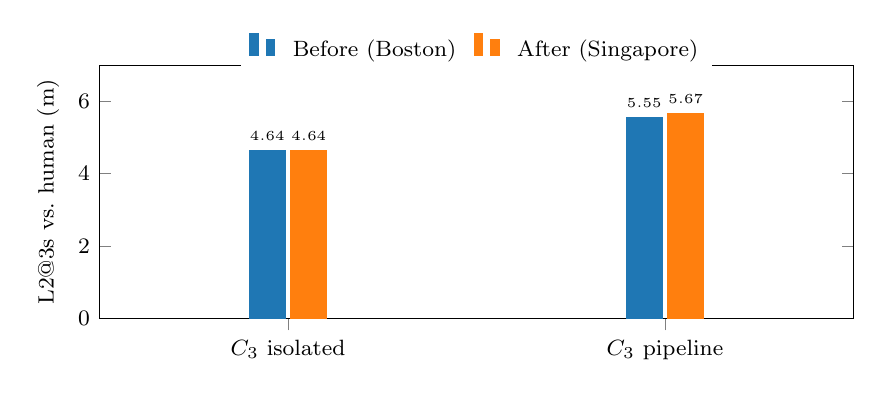
\begin{tikzpicture}
\begin{axis}[
  width=0.92\columnwidth, height=4.8cm,
  ybar=2pt, /pgf/bar width=13pt, ymin=0, ymax=7.0,
  ylabel={L2@3s vs.\ human (m)},
  symbolic x coords={iso, pipe}, xtick=data,
  xticklabels={$C_3$ isolated, $C_3$ pipeline},
  tick label style={font=\footnotesize}, label style={font=\footnotesize},
  enlarge x limits=0.5,
  legend style={at={(0.5,1.15)}, anchor=north, legend columns=2,
                draw=none, font=\footnotesize, column sep=1ex},
  nodes near coords, nodes near coords style={font=\tiny,
        /pgf/number format/fixed, /pgf/number format/precision=2},
]
\addplot[fill=beforeblue, draw=beforeblue]
  coordinates {(iso,4.64) (pipe,5.55)};
\addplot[fill=afterorange, draw=afterorange]
  coordinates {(iso,4.64) (pipe,5.67)};
\legend{Before (Boston), After (Singapore)}
\end{axis}
\end{tikzpicture}
\caption{Cascade signature on planning. The metric of $C_3$ in isolated mode stays
fixed while its metric in pipeline mode moves.}
\label{fig:cascade}
\end{figure}

\begin{figure}[htbp]
\centering
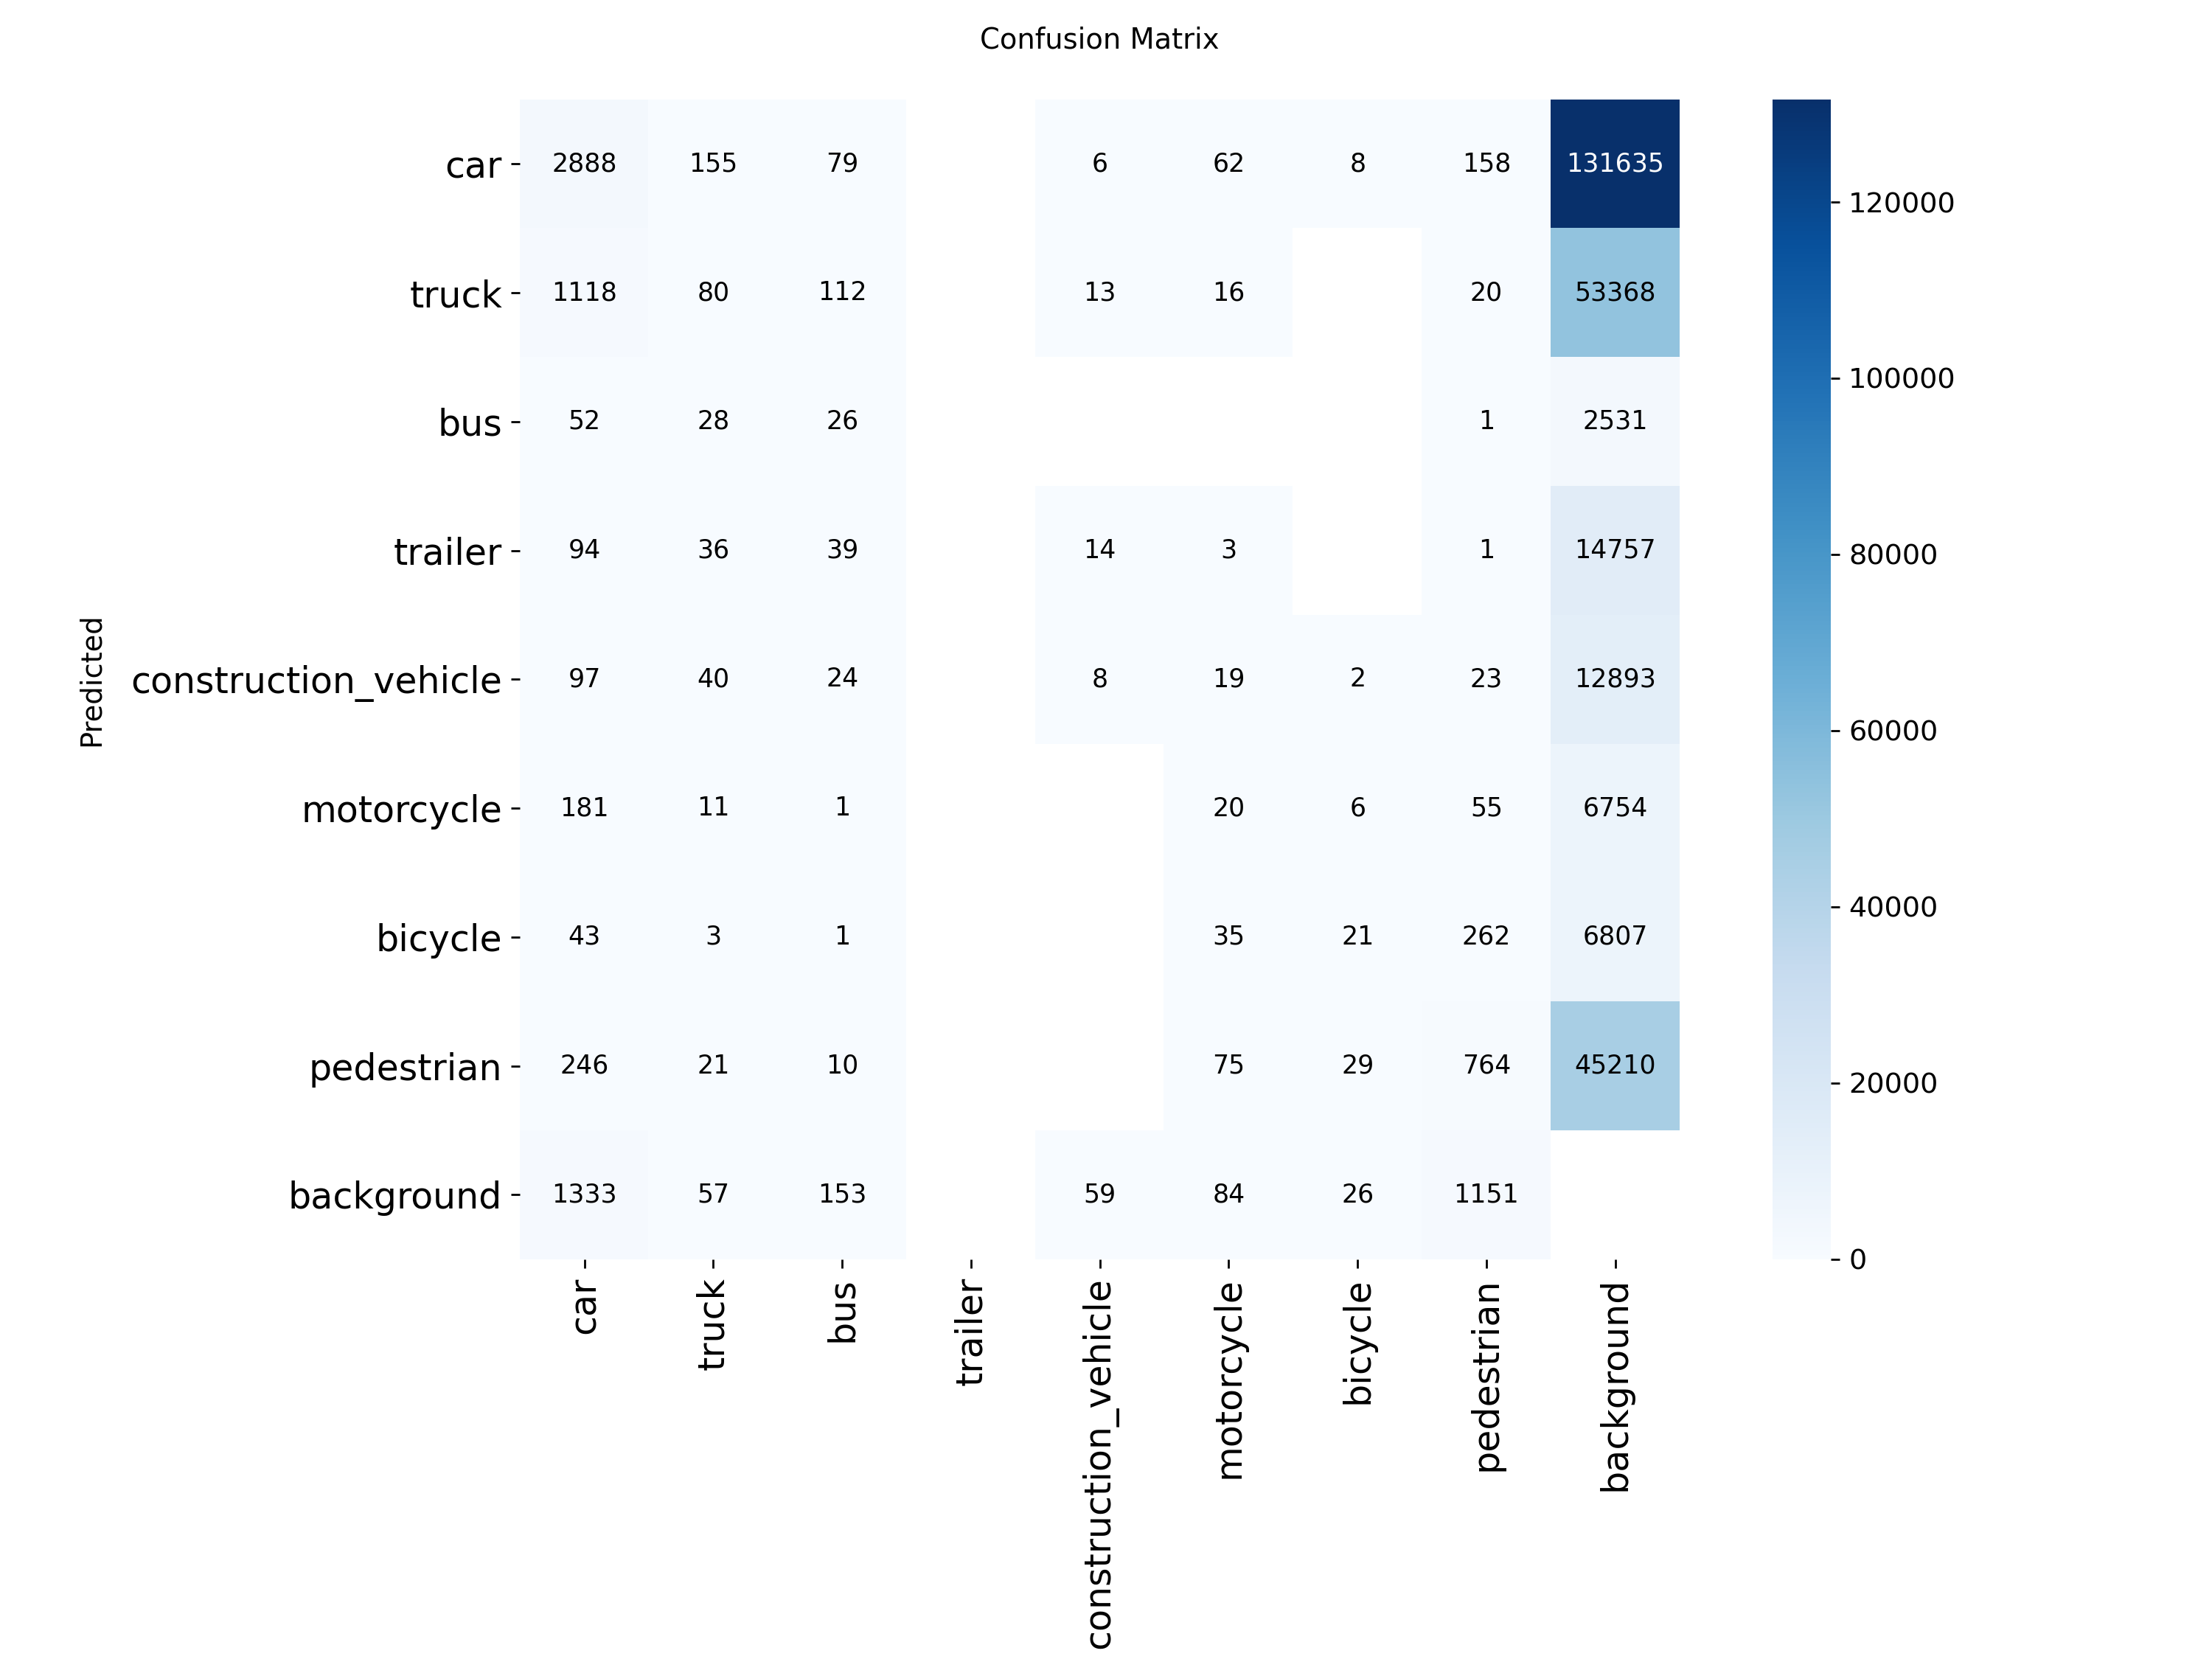
\includegraphics[width=0.92\columnwidth]{figures/fig06_confusion_boston.png}
\caption{Confusion matrix of the Boston-trained $C_1$ on full trainval.}
\label{fig:confusion}
\end{figure}

\subsection{The Campaign}
\label{sec:res-campaign}
\emph{Objective.} Determine how often entangled enhancement occurs, and how
strongly, when the retraining configuration is varied rather than fixed.

The reference update is a single point in a large space of possible updates.
Table~\ref{tab:campaign} reports all $15$ updates of the campaign
(Section~\ref{sec:campaign}), and three patterns emerge.

First, the detector improves on its own metric in \emph{every} update, with
$\delta_1 > 0$ in all $15$, and prediction improves as well, with $\Delta_2 < 0$
in all $15$. Fine-tuning on the new city genuinely sharpens $C_1$ across the whole
campaign.

Second, and most importantly, this is enough to observe \emph{entangled
enhancement directly}: in $6$ of the $15$ updates $\delta_1 > 0$ while
$\Delta_3 > 0$, i.e. the detector improves yet the planner degrades. The six span
a range of severities, from a marginal $+0.008$~m up to a material $+0.193$~m. No
class re-balancing is required to reach this condition, which arises in the ordinary
campaign.

Third, the direction of the effect on planning is campaign-dependent. The
planner is worse ($\Delta_3 > 0$) in $6$ updates and better ($\Delta_3 < 0$) in
the other $9$. The training configuration does not predict which updates degrade
the planner. A rule based on the detector alone is therefore not sufficient, and
the update has to be checked at the downstream models (Section~\ref{sec:cara}).

\begin{table}[htbp]
\caption{The $15$-update retraining campaign on \texttt{singapore\_val}
($n=2{,}020$ frames). A positive $\delta_1$ marks an improved detector, a negative
$\Delta_2$ an improved prediction, and a positive $\Delta_3$ a worse planner. The
shift column is the plan shift in metres. ``ent.\ enh.'' marks entangled
enhancement ($\delta_1>0$ with $\Delta_3>0$) and ``helped'' marks $\Delta_3<0$.
Every update has $\delta_1>0$.}
\label{tab:campaign}
\centering
\renewcommand{\arraystretch}{1.15}
\setlength{\tabcolsep}{3.5pt}
\footnotesize
\begin{tabular}{@{}lrrrrrl@{}}
\toprule
\textbf{Update} & \textbf{data} & \textbf{$\delta_1$} & \textbf{$\Delta_2$} & \textbf{$\Delta_3$} & \textbf{shift} & \textbf{outcome} \\
\midrule
Full, 10\,ep, s1     & full & $+0.119$ & $-2.17$ & $+0.124$ & $1.05$ & \textbf{ent.\ enh.} \\
Full, 10\,ep, s2     & full & $+0.122$ & $-2.28$ & $+0.193$ & $1.02$ & \textbf{ent.\ enh.} \\
Full, 10\,ep, s3     & full & $+0.129$ & $-2.15$ & $+0.187$ & $0.92$ & \textbf{ent.\ enh.} \\
Half, 10\,ep, s1     & half & $+0.114$ & $-2.55$ & $-0.121$ & $1.35$ & helped \\
Half, 10\,ep, s2     & half & $+0.120$ & $-2.71$ & $-0.230$ & $1.19$ & helped \\
Half, 10\,ep, s3     & half & $+0.106$ & $-1.77$ & $-0.151$ & $1.46$ & helped \\
Quarter, 10\,ep, s1  & qtr  & $+0.121$ & $-2.71$ & $+0.073$ & $0.79$ & \textbf{ent.\ enh.} \\
Quarter, 10\,ep, s2  & qtr  & $+0.113$ & $-1.29$ & $-0.093$ & $0.78$ & helped \\
Quarter, 10\,ep, s3  & qtr  & $+0.101$ & $-2.82$ & $+0.008$ & $1.00$ & \textbf{ent.\ enh.} \\
Full, 5\,ep, s1      & full & $+0.138$ & $-1.08$ & $-0.095$ & $0.89$ & helped \\
Full, 5\,ep, s2      & full & $+0.122$ & $-1.88$ & $-0.130$ & $1.22$ & helped \\
Full, 5\,ep, s3      & full & $+0.130$ & $-1.08$ & $-0.041$ & $0.92$ & helped \\
Full, 20\,ep, s1     & full & $+0.142$ & $-2.59$ & $+0.037$ & $1.37$ & \textbf{ent.\ enh.} \\
Full, 20\,ep, s2     & full & $+0.126$ & $-1.77$ & $-0.083$ & $1.50$ & helped \\
Full, 20\,ep, s3     & full & $+0.130$ & $-2.44$ & $-0.020$ & $1.20$ & helped \\
\bottomrule
\end{tabular}
\end{table}

\subsection{Robustness to Class Imbalance}
\label{sec:res-balanced}
\emph{Objective.} Test whether entangled enhancement is an artifact of class
imbalance in the training data rather than a property of the pipeline.

The campaign already yields entangled enhancement without any intervention on the
training data. A natural question is whether the effect is an artifact of the
residual class imbalance visible in Fig.~\ref{fig:confusion}, where rare classes
are still confused with background. To test this, we repeat the campaign with a
class-balanced training split. Images containing rare classes are oversampled so
that the per-class instance distribution flattens, with a repeat factor
$(n_{\max}/n_c)^{p}$ per class $c$ clipped to
$[1,12]$, while the validation split is left untouched so metrics stay comparable.
We run two balance strengths ($p \in \{0.5, 1.0\}$), two training lengths
($10$ and $20$ epochs), and three seeds, giving $12$ updates.

The effect persists under class balancing. Across the $12$ updates the
detector still improves in every case ($\delta_1 > 0$ in $12/12$), and entangled
enhancement appears in $4$ of the $12$. Three occur at $p{=}0.5$
(\texttt{ep10\_s3}, \texttt{ep20\_s1}, \texttt{ep20\_s2}, with $\delta_1$ up to
$+0.143$ and $\Delta_3$ up to $+0.139$~m) and one at $p{=}1.0$
(\texttt{ep20\_s1}, $\delta_1{=}+0.125$, $\Delta_3{=}+0.075$~m). Entangled enhancement appears at
both balance strengths and at both training lengths, with three of the four cases
occurring at $20$ epochs. Rebalancing the rare classes therefore does not remove
the effect. The condition is
not an artifact of the residual class imbalance but a property of the pipeline
under domain-shift retraining.

\subsection{Evaluation of CARA's Drift Screen}
\label{sec:res-gate}
\emph{Objective.} Determine whether the low-cost drift score of CARA
predicts the downstream effect that only the full pipeline reveals.

For each of the $15$ updates we compute the drift score of the updated detector
against the original detector on the audit scenes. Ranked against the plan shift,
the score is a moderate predictor of \emph{how much} the plan moves, with a rank
correlation of $\approx 0.56$ (Fig.~\ref{fig:drift-scatter}). The score does not
separate the updates that worsen the planning metric ($\Delta_3 > 0$) from the
rest. Its AUROC for this classification is $\approx 0.48$, which is the value
expected from a random ranking. Every retrained detector improved
consistently, and all scores therefore fall in a narrow band ($0.05$ to $0.08$) in which the two
groups interleave. The drift screen therefore indicates the \emph{magnitude} of
downstream disturbance but not its \emph{direction}, which makes it a filter that
prioritizes updates for the full admission procedure of
Algorithm~\ref{alg:cara} rather than a standalone rule.

\begin{figure}[htbp]
\centering
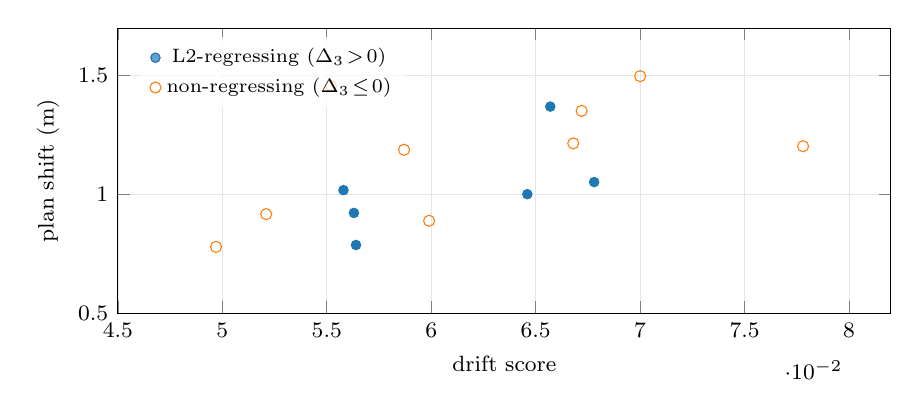
\begin{tikzpicture}
\begin{axis}[
  width=0.94\columnwidth, height=5.2cm,
  xlabel={drift score}, ylabel={plan shift (m)},
  xmin=0.045, xmax=0.082, ymin=0.5, ymax=1.7,
  tick label style={font=\footnotesize}, label style={font=\footnotesize},
  legend style={at={(0.03,0.97)}, anchor=north west, font=\scriptsize,
                draw=none, fill=white, fill opacity=0.7, text opacity=1},
  grid=both, grid style={line width=0.2pt, draw=gray!20},
]
% L2-regressing updates (Delta3>0): filled circles
\addplot[only marks, mark=*, mark size=1.7pt, beforeblue] coordinates {
  (0.0678,1.052) (0.0558,1.018) (0.0563,0.922) (0.0564,0.787)
  (0.0646,1.001) (0.0657,1.370)};
% non-regressing updates (Delta3<=0): open circles
\addplot[only marks, mark=o, mark size=2pt, afterorange] coordinates {
  (0.0672,1.352) (0.0587,1.188) (0.0552,1.456) (0.0497,0.779) (0.0700,1.498)
  (0.0778,1.203) (0.0599,0.889) (0.0668,1.215) (0.0521,0.917)};
\legend{L2-regressing ($\Delta_3\!>\!0$), non-regressing ($\Delta_3\!\le\!0$)}
\end{axis}
\end{tikzpicture}
\caption{Drift score vs.\ plan shift over the $15$ updates. Drift tracks the
magnitude of plan movement, but the two groups interleave.}
\label{fig:drift-scatter}
\end{figure}

\subsection{Evaluation of CARA's Admission Rule}
\label{sec:res-admission}
\emph{Objective.} Determine whether the drift score, used as a binary admit-or-hold
rule, separates the updates that regress the planning metric from the rest.

We label an update ``L2-regressing'' when it worsened the trajectory-agreement
metric ($\Delta_3 > 0$). Of the $15$ updates, $6$ are L2-regressing and $9$ are not.

As a thresholded decision the rule is weak, as Table~\ref{tab:admission}
shows. At a conservative threshold every update is held, and no L2-regressing update is therefore
admitted (recall $1.0$) but no update is admitted at all (specificity $0$), which
is safe but provides no discrimination. The best balanced operating point still
catches every L2-regressing update (recall $1.0$) but admits only two of nine
non-regressing ones (specificity $0.22$), at precision $0.46$. The drift screen can
be tuned to catch every L2 regression, but at the cost of holding most other
updates too. The two planning clauses of Algorithm~\ref{alg:cara} disagree here,
which is the point. The original pipeline had a $2\%$ collision rate, and every
updated model drove it to zero, and the collision-rate clause would therefore admit all
$15$. The L2 clause, in contrast, holds the six $\Delta_3>0$ updates.
CARA holds those six on L2 even though their collision rate improved, and neither
clause alone is a safe gate. CARA does not reduce the assessment to a single
admit-or-hold decision. CARA reports the change at every downstream model, and the
disagreement between the two metrics of $C_3$ is therefore visible to the
maintainer, who can then decide whether to hold the update or to retrain the
downstream models together with it.

\begin{table}[htbp]
\caption{CARA drift-rule decisions against ground truth ($\Delta_3 > 0 =$
L2-regressing), on the $15$ full-trainval updates ($6$ L2-regressing, $9$ not).
The held-out row tunes the threshold on a $7$-update tune split and reports on
the untouched $8$-update test split.}
\label{tab:admission}
\centering
\renewcommand{\arraystretch}{1.2}
\setlength{\tabcolsep}{5pt}
\begin{tabular}{@{}lcccccc@{}}
\toprule
\textbf{Threshold} & \textbf{TP/FP/FN/TN} & \textbf{Rec.} & \textbf{Spec.} & \textbf{Prec.} & \textbf{F1} \\
\midrule
Strict (hold all)      & $6/9/0/0$ & $1.00$ & $0.00$ & $0.40$ & $0.57$ \\
Balanced              & $6/7/0/2$ & $1.00$ & $0.22$ & $0.46$ & $0.63$ \\
Held-out (test)        & $3/3/0/2$ & $1.00$ & $0.40$ & $0.50$ & $0.67$ \\
\bottomrule
\end{tabular}
\end{table}

We interpret these results conservatively. The threshold is chosen on a $7$-update
tune half and applied to the untouched $8$-update test half. The reported
operating point is therefore not fitted on the data it is scored against. On that held-out test the rule still catches every
L2-regressing update (recall $1.0$) but keeps a low specificity ($0.40$),
confirming that the drift screen is a prioritization filter, not a decision
rule. With only $8$ test updates the estimates are wide: Wilson $95\%$ intervals
are $[0.44, 1.00]$ recall, $[0.12, 0.77]$ specificity, and $[0.19, 0.81]$
precision, and they are indicative rather than tight. The full admission procedure of
Algorithm~\ref{alg:cara} remains the reliable decision, and the drift screen serves
as its low-cost first filter that never misses an L2-regressing update.

\subsection{Training Diagnostics}
Both fine-tunes converged within their epoch budgets with monotone loss
decay, as Fig.~\ref{fig:curves} shows for the Boston run. The box,
classification, and distribution-focal losses decrease on both the train and
validation splits, while precision, recall, and mAP@50 increase, with mAP@50
rising from $0.116$ at epoch 1 to $0.137$ at epoch 10. A single update, comprising the
fine-tune and both evaluations, costs about $24$ GPU-minutes, and the whole
$15$-update campaign ran in about six GPU-hours. That budget is far below the cost
of training an end-to-end planner~\cite{sun2024sparsedrive}, which is what makes a
campaign of repeated retraining feasible.

\begin{figure}[htbp]
\centering

\includegraphics[width=\columnwidth]{figures/fig04_boston_curves.png}
\caption{YOLOv11n $C_1$ Boston fine-tune training curves.}
\label{fig:curves}
\end{figure}

% ============================================================================
\section{Discussion}
\label{sec:implications}
% ============================================================================
We explain the mechanism behind the non-monotone cascade and place CARA among
related maintenance techniques.

\subsection{Why the Cascade Is Non-Monotone}
Under the Boston-trained $C_1$, the planner's inputs were substantially displaced
($\Gamma_2 = 6.81$~m) in a regime whose errors the proposal-and-score rules
absorbed. Missed or grossly misplaced agents leave the proximity penalty
inactive, and the planner therefore follows its kinematic prior, which on these scenes
approximated the human trajectory. The updated $C_1$ relocated detections near
their true positions and re-activated the penalty with correctly anchored but
coarse (zero-velocity) forecasts, causing the planner to react to obstacles it
had previously ignored. Downstream models can thus absorb upstream error,
and, symmetrically, upstream improvement can expose masked downstream
sensitivity. An updated model therefore cannot be admitted on its own
output alone.

\looseness=-1
This mechanism also cautions against a literal interpretation of the planning
metric. The collision rate \emph{fell}, from $2\%$ under the original model to
zero after retraining, even as L2 rose, and the higher L2 of the reference case
arises because the improved detector caused the planner to react to real agents
rather than follow a kinematic prior that happened to track the recorded human
path. That behaviour is the ego-forecasting shortcut of nuScenes open-loop
L2, under which perception-agnostic prediction is
competitive~\cite{zhai2023rethinking} and open-loop error is weakly tied to
closed-loop quality~\cite{codevilla2018offline}. A regression on this metric may
therefore mark a \emph{safer} planner that scores worse on a measure rewarding
ignored perception, and the planning metrics here should therefore be read as reduced
trajectory agreement, not an established safety regression, and a closed-loop or
NAVSIM-style metric~\cite{dauner2024navsim} is the appropriate safeguard.

\subsection{CARA Among Related Maintenance Techniques}
The findings give three maintenance rules that CARA (Section~\ref{sec:cara})
enforces directly. An update must not be admitted on the updated model's own
metric, and admission must not stop at the next model, because the
entangled-enhancement cases are exactly those in which $C_1$ improved and $C_2$
improved while $C_3$ degraded. A maintenance policy should also assess several
candidate updates rather than trust one, because the effect on planning varies
across updates.

CARA is one of several complementary techniques for these rules, not a
replacement for them. Regression-constrained retraining such as
positive-congruent training~\cite{yan2021pctraining} and backward-compatible
training~\cite{shen2020bct} \emph{reduces} the cascade at its source by
constraining the update. Uncertainty-propagating
interfaces~\cite{ivanovic2022propagating} \emph{absorb} the residual by passing
distributions instead of point estimates across the perception--prediction
boundary. Between-stage data validation~\cite{breck2019data} \emph{monitors} the
interface in production. CARA adds the missing \emph{admission} step that measures
the downstream cascade directly before an update is deployed, and its low-cost
drift screen (Section~\ref{sec:cara-frontend}) can operate alongside
the same production monitors.

% ============================================================================
\section{Related Work}
\label{sec:related}
% ============================================================================

\subsection{End-to-End Driving and Its Maintenance Limits}
UniAD put detection, tracking, mapping, motion forecasting, occupancy
prediction, and planning into a single planning-oriented
network~\cite{hu2023uniad}. VAD replaced dense rasterized scene
representations with vectorized ones for efficiency~\cite{jiang2023vad}.
SparseDrive introduced fully sparse scene representations and reported the
resource profile of the flagship systems: $7.2\times$ faster training and
$5\times$ faster inference than UniAD, whose training takes about 144
GPU-hours~\cite{sun2024sparsedrive}. The main survey of the field lists
interpretability, causal confusion, and robustness under distribution shift
as open challenges, and it does not treat component-level maintenance or
retraining policy at all~\cite{chen2024e2esurvey}.

A recent end-to-end repair literature addresses maintenance directly. CorrectAD
builds a self-correction loop that diagnoses failures, generates targeted
training video with a diffusion model, and fine-tunes the entire end-to-end planner
on old plus new data, correcting 62.5\% of failure cases on
nuScenes~\cite{ma2025correctad}. R2SE avoids full-model retraining by freezing
the generalist model and training reinforcement-learned low-rank adapter
specialists on failure regions, motivated by the catastrophic forgetting that
naive fine-tuning causes~\cite{liu2025r2se}. Both reintroduce pipeline structure
to make maintenance tractable, which motivates the pipeline architecture adopted
in this work.

\subsection{Evaluation of Driving Systems}
Our planning metric is open-loop displacement error on nuScenes, and the
limits of this protocol are well documented. Codevilla et al. showed as early
as 2018 that offline prediction error correlates only weakly with actual
closed-loop driving quality~\cite{codevilla2018offline}. Zhai et al. found
that a trivial MLP using only ego state, with no perception at all, matches
perception-based end-to-end methods on nuScenes open-loop
L2~\cite{zhai2023rethinking}. Dauner et al. showed that open-loop
ego-forecasting and closed-loop driving are misaligned tasks, and that a
largely rule-based planner, PDM-Closed, outperformed learned
planners~\cite{dauner2023parting}. Their later NAVSIM benchmark provides
short-horizon non-reactive metrics that align far better with closed-loop
performance~\cite{dauner2024navsim}. These critiques target open-loop metrics
used to \emph{rank} architectures. Our use is differential (the same unchanged
planner, same scenes, one upstream change), and much of that weakness therefore cancels,
and we report collision rate alongside L2 and revisit the caveat in
Section~\ref{sec:implications}.

\subsection{Model Updates, Regression, and Interface Compatibility}
What we measure at system scale has per-sample analogues in the model-update
literature. Yan et al. showed that model updates cause negative flips, samples
the old model handled correctly that the new model gets wrong, at rates of
4--5\% even between equal-accuracy retrains of identical architectures, and
they proposed positive-congruent training with focal distillation to suppress
them~\cite{yan2021pctraining}. The backward-compatible training of Shen et al.
constrains a new upstream representation model so that unchanged downstream
consumers keep working~\cite{shen2020bct}, which is the same situation as
updating $C_1$ beneath an unchanged $C_2$ and $C_3$. On the monitoring side, the data
validation system of Breck et al. runs two-sample distribution tests between
pipeline stages in production~\cite{breck2019data}. On a nuScenes
detector--tracker--predictor stack nearly the same shape as ours, Ivanovic et
al. showed that propagating state uncertainty across the
perception--prediction interface, instead of passing point estimates, improves
forecasting by a wide margin~\cite{ivanovic2022propagating}. These works
provide mitigation techniques. This paper contributes the complementary
controlled measurement of the cascade that such techniques are intended to
mitigate.

\subsection{Reliability Modeling of Machine Learning Systems}
The technical-debt analysis of Sculley et al. introduced CACE, unstable data
dependencies, and correction cascades as qualitative failure modes of ML
systems~\cite{sculley2015hidden}. The base paper for this work, Wang and
Machida~\cite{wang2024compsac}, formalized imperfect retraining of a
two-model machine learning system as a continuous-time Markov chain, named entangled
enhancement, and compared progressive and conservative maintenance policies.
Their follow-on work casts the same problem as an availability--continuity
trade-off~\cite{wang2025issre}. Both are analytical models whose state space
grows as $2^N$ for $N$ components, and both are calibrated on synthetic
transition rates. This paper provides an empirical counterpart. The isolation
property we verify empirically is the property their state factorization assumes, and
the coupling factor we propose (Section~\ref{sec:cara}) is a measured statistic
that can replace those synthetic rates.


% ============================================================================
\section{Conclusion}
\label{sec:conclusion}
% ============================================================================
We presented a controlled study of single-model retraining in a
perception--prediction--planning pipeline under a geographic domain shift. Using
the two-mode measurement with a verified isolation control on the full nuScenes
trainval split ($2{,}020$ evaluation frames), and running a campaign of $15$
retraining updates rather than a single event, we found that retraining $C_1$
disturbs the downstream plan in every case. The retrained detector improves on
its own metric in all $15$ updates, and yet in $6$ of them the planner's
trajectory-agreement metric worsens at the same time. Entangled enhancement is
therefore not only an analytically modeled hazard but an observable one in a real
AV pipeline, reached without any data-balancing intervention. The two planning
metrics moreover \emph{diverge}. On the reference update the collision rate
improved to zero while L2 agreement worsened. Together these results
show that model-level validation, and any single-metric check on the system
output, is insufficient for safe maintenance of a machine learning system, since each of those six updates
would have passed a review of $C_1$ alone and a review of the collision rate alone. We proposed the CARA admission method for
maintaining such pipelines and evaluated its drift screen on a
held-out split. The drift screen tracks the magnitude of downstream disturbance
(Spearman $\approx 0.56$) but does not classify harm on its own (AUROC $\approx
0.48$), and it is therefore a prioritization filter for the full admission
procedure rather than a standalone decision rule. The broader contribution is
methodological. Cascade effects can be measured under exact controls, but only in
an architecture that exposes the connections between its models.

\bibliographystyle{IEEEtran}
\bibliography{references}
\end{document}
